\documentclass[conference]{IEEEtran}
\IEEEoverridecommandlockouts
% The preceding line is only needed to identify funding in the first footnote. If that is unneeded, please comment it out.
\usepackage{amsmath,amssymb,amsfonts}
\usepackage{algorithmic}
\usepackage{graphicx}
\usepackage{textcomp}
\usepackage{xcolor}
\usepackage{color}
\usepackage{soul}
\usepackage{hyperref}
\usepackage[backend=biber, style=ieee, url=false]{biblatex}
\usepackage{varioref}
\usepackage{hyperref}
\usepackage{cleveref}
\usepackage{booktabs,caption}
\usepackage[flushleft]{threeparttable}
\renewcommand*{\bibfont}{\footnotesize}
\setlength{\biblabelsep}{\labelsep}
\setlength{\bibitemsep}{\IEEEbibitemsep}

\addbibresource{bibliography.bib}

\begin{document}

\title{Netflix QoExtension - A Tool for Conducting Ecologically Valid Experiments}

\author{\IEEEauthorblockN{Rafał Figlus}
\IEEEauthorblockA{\textit{rfiglus@agh.edu.pl} \\
\textit{AGH University of Science and
Technology, Institute of
Telecommunications
Kraków, Poland}\\
\\
}

%\and
%\IEEEauthorblockN{{}}
%\IEEEauthorblockA{\textit{} \\
%\textit{}\\
%\\}

%\and
%\IEEEauthorblockN{{}}
%\IEEEauthorblockA{\textit{} \\
%\textit{}\\
%\\}

%\and
%\IEEEauthorblockN{{}}
%\IEEEauthorblockA{\textit{} \\
%\textit{}\\
%\\}

%\and
%\IEEEauthorblockN{{}}
%\IEEEauthorblockA{\textit{} \\
%\textit{}\\
%\\}
}
\maketitle

\begin{abstract}
    This paper describes Netflix QoExtension, a tool designed to facilitate ecologically valid experiments on the Netflix video streaming platform by enabling researchers to manipulate video quality of content selected by subjects based on their preferences. It enables researchers to create experiment sessions of varying duration, using any of the movies or TV shows available on Netflix.
\end{abstract}

\begin{IEEEkeywords}
    Quality Of Experience; Netflix; Ecological Validity; Chrome Extension;
\end{IEEEkeywords}

\section{Introduction}
\label{sec:Introduction}
    A significant portion of research in the field of Quality of Experience (QoE) relies on the fundamental methodology outlined in the ITU recommendations, such as BT.500 \cite{BT.500-14} or P.913 \cite{ITU-T-P.913}. A typical experiment consists of a series of video stimuli presented to the subject. After each stimulus quality score is collected from the subject, the process is repeated multiple times using numerous videos sharing similar or the same content. 
    
    One critique of the experiments described in \cite{BT.500-14, ITU-T-P.913} is the repeatability of the task. From \cite{brain} we know that the human brain functions differently if a task, such as asking a simple question, is repeated multiple times. This can negatively impact the accuracy of the quality scores they provide. 
    Additionally, this approach focuses mainly on perceived video quality. No other factors that may influence subject's overall QoE in a real-world setting, such as interest or immersion, are taken into account. The stimuli presented are typically of short length and are not perceived by the subjects as entertaining. Therefore, such experiment is not considered ecologically valid as it does not reflect real life conditions in which multimedia are consumed by users.

    % Claims and contribution
    In this paper we claim that it is possible to conduct QoE experiments in ecologically valid environments where objective metrics of video playback and subjective scores can be collected in accordance to \cite{BT.500-14}. 
    Therefore, we propose experiment utilizing Netflix streaming platform where subject can select content aligning with their interest. 

    Our contribution is design and development of \verb|Netflix QoExtension| - a Chrome browser extension that utilizes Netflix web application and its features such as playback performance statistics and possibility to display video encoded with different bitrate values. 
% Introduction - end

\section{Related work}
\label{sec:related_work}
    % Intorduction to literature-study
    There have been attempts to research QoE using more ecologically valid methodologies. Even though \textit{ecological validity} \cite{kihlstrom2021ecological} is not mentioned directly, authors try to conduct experiments resembling real-life scenarios which they achieve using different methods.
    
    % Description of custom YT-like research app
    In \cite{custom_yt_like_app} researchers came up with an application resembling popular video platform. Subjects had the possibility to watch videos from a predefined set of 32 videos that were encoded to 5 different quality profiles. Duration of the videos was ranging from 1.5 to 3 minutes and some of them were cut from longer sequences. 
    Study was focused on behavior of subjects exposed to different video qualities and events such as stalling. 
    Real purpose of the study was not revealed to subjects until the end of experiment and no subjective video quality ratings were collected during the examination.
    Although such methodology ensures higher level of ecological validity, due to freedom of content choice and availability of basic actions such as video seeking, pausing or skipping the video, it does not reflect full experience of interacting with video platform like YouTube or Netflix as the number of available videos is significantly smaller. Also content selected by experimenters might not be interesting in the eyes of the subjects. 
    This stands in opposite to our intentions for ecologically valid experiment where subjects can select any content they want from service such as YouTube or Netflix. Another key feature is subjects' engagement in the content which is difficult to achieve with short video sequences.
    
    % Description of YouSlow
    Researchers in \cite{you_slow} utilized YouTube video platform in full capacity by creating \textit{YouSlow} - a web browser extension capable of monitoring YouTube playback metrics and various events such as start-up latency, rebufferings and bitrate changes.
    Methodology taken in the study focuses on examination of influence of mentioned events on video abandonment.
    Presented methodology does not include examination of user behavior nor subjective video quality scores.
    However, experiment design ensures high level of ecological validity by allowing subjects to interact with YouTube naturally. 
    Moreover, experimenters were in no control of video quality or events occurring during video playback which on the other hand stands in opposite to our intentions where experimenters can design experiment scenarios and have control over its execution.
    
    % Description of YoMoApp 
    % 1. technical paper
    % 2. unsupervised field study
    Similar approach was presented in \cite{yo_mo_app_technical} where researchers came up with YoMoApp - an application for mobile Android devices utilizing YouTube in full capacity. 
    Application was designed with intention to conduct client-side measurements of YouTube performance in mobile networks. YoMoApp allowed for collecting objective metrics such as player state/events, buffer and video quality.
    Study presents subjective laboratory experiment conducted in order to prove accuracy of designed tool.
    Subjects were imposed to watch 2 minutes long videos exposed to 5 different network conditions enforced by intermediate router. After watching each video exposed to one of the network conditions subjects were asked to rate watching experience in form of e.g. overall experience, impact of initial delay, stalling and video quality on a ACR \cite{ITU-T-P.913} MOS \cite{P.800} scales.
    Despite the utilization of YouTube video platform, subjects were forced to watch short videos selected by experimenters which degrades the level of ecological validity. 
    Presented experiment design resembles standard approach defined in \cite{BT.500-14}. 
    In opposite to previous study researchers were in more control over the experiment.
    Improved version of \textit{YoMoApp} was used in \cite{yo_mo_app_unsupervised_qoe_field_study} where unsupervised field study was conducted.
    
    % Description of YTCrowdMon
    Researchers in \cite{are_you_still_watching_YT_CrowdMon} went one step further in comparison to \cite{you_slow} and \cite{yo_mo_app_technical}, \cite{yo_mo_app_unsupervised_qoe_field_study} and examined not only streaming performance but also user behavior. \textit{YTCrowdMon} - a web browser extension capable of taking measurements not only in YouTube but also Netflix and Amazon Prime Video was developed.
    Study achieved high level of ecological validity allowing subjects using different video services but experimenters were in no control over the quality of videos. Additionally no subjective scores were collected.
% Realted Work - end

\section{NetflixQoExtension - Concept and description}
In order to achieve high level of ecological validity we have to utilize one of the popular video services available. We have selected Netflix for couple of reasons. It is a popular service in Poland, it provides video playback performance statistics and another feature which is ability to manipulate presented video bitrate.
In order to fully utilize information and features available in Netflix we designed and developed \verb|Netflix QoExtension| - a Chrome web browser extension.

Primary goal of the study is to investigate correlation between VMAF \cite{VMAF} and subjective quality. 
Subjects come to the laboratory and watch content selected by themselves in different video quality conditions imposed by our tool. 
Throughout the experiment, in configured time intervals subjects are asked to score audio-visual quality of what is being presented to them.

Outline of features and data flow of the tool is presented in fig. \ref{Figure:fig_features}.
Netflix QoExtension works within Chrome browser and interacts with Netflix web application and our backend server where captured data are stored in a database. More features are described in the following sections.

\begin{figure}[h]
      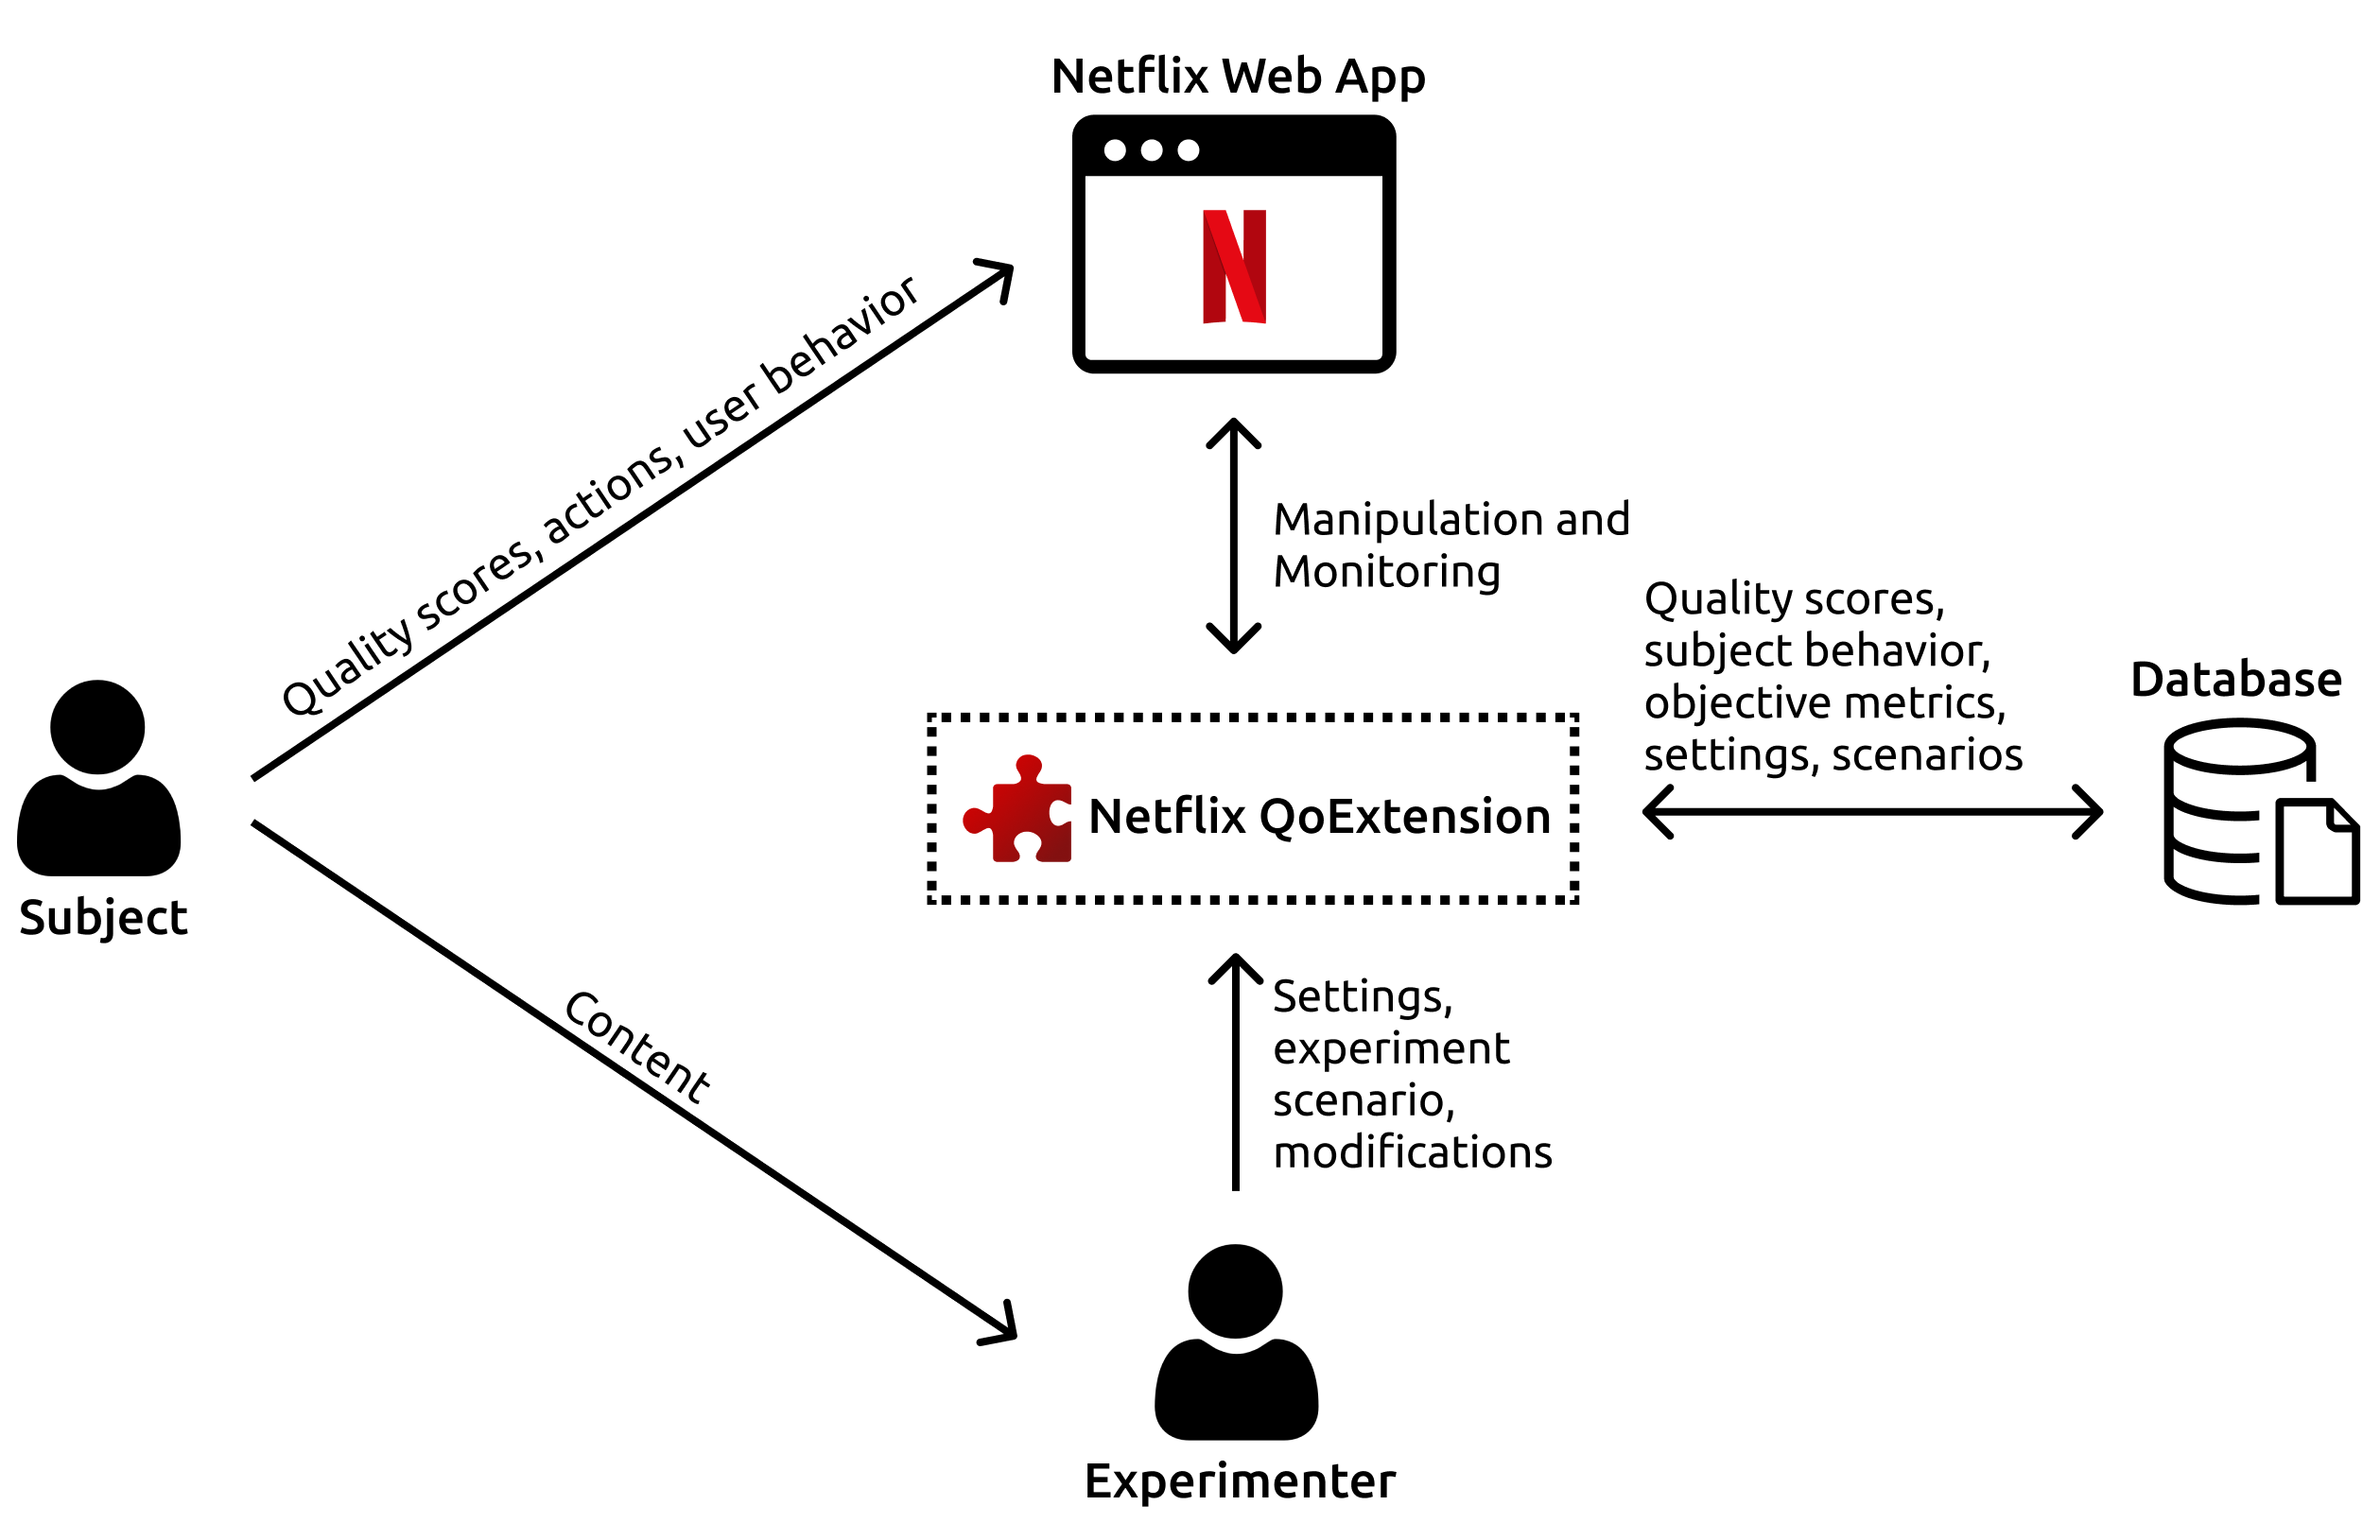
\includegraphics[width=3.38in]{assets/NetflixQoExtensionV2.png}
      \caption{Features and data flow}
      \label{Figure:fig_features}
\end{figure}

\subsection{Experiment preparation}
Content selected by subjects has to be known to experimenters before running actual experiment due to number of factors. We want each subject to be exposed to uniform distribution of VMAF values. However Netflix allows only for selecting video quality by selecting bitrate values the video is encoded with. According to our research and observations each available bitrate value corresponds directly to a VMAF value. Therefore video URLs have to be known in advance in order to execute bitrate to VMAF mapping process for each video the subject wishes to watch. 
The process results in generating a configuration which is later used to start experiment.

\subsection{Quality changes}
By default Netflix web application does not allow manually fixing bitrate values. This is available thanks to \cite{netflix-1080p} and their modifications of cadmiumPLayercore - Netflix's video player implementation in JavaScript.
Quality changes imposed by the extension apply only to the content being buffered. A change of quality is not immediately seen on the screen but as playback progresses new content is being buffered. Thanks to that we can achieve seamless transitions between qualities without screen flickering or rebuffering indicating changes which could influence subject's behavior and judgement.
By default Netflix's JavaScript implementation of video player - cadmiumPlayercore is configured to buffer up to 240 seconds of video but the extension allows for modification of that value.
As video playback progresses the buffer gets emptied and new video chunks are downloaded from CDN servers. 

One limitation related to quality changes is that subjects are deprived of pausing and seeking the video as it would negatively affect the distribution of planned video qualities. In current version we could not afford that due to limited number of subjects invited to the laboratory experiment. Additionally subjects do not have full freedom of interacting with Netflix platform for example in form of searching through available content which has to be known before coming to the laboratory. 

For every video in Netflix there are different sets of bitrates available. On quality change, the extension selects bitrate value closest to the value defined in pattern. This causes deviations from original pattern provided in configuration file. In future versions of the extension one could implement different patterns of quality changes e.g descending or random.

\subsection{Objective playback metrics}
Netflix exposes playback statistics menu containing various information on current audio-video playback such as movie id, player state, current video resolution and VMAF, buffer state and more.  At the start of playback extension programatically invokes the statistics by dispatching special keyboard key event. After that HTML DOM tree is analyzed to search for element holding the statistics. Said element is periodically scanned in order to fetch required data which are then send to backend side and stored in database.

According to our observations information displayed by the element are updated in time intervals of approximately 1 second which puts constraint on measurement accuracy.
Another limitation is related to VMAF value displayed as part of objective metrics as it describes entire video encoded with particular bitrate. It puts a significant constraint on accuracy due to variability in scenes characteristics within a video. Highly dynamic scenes encoded with particular bitrate should obtain lower VMAF scores in comparison to less dynamic scenes.
% oglna mysl jest taka - sceny/klatki z duza dynamika/duzo szumu/duzo roznych czestotliwosci maja wiecej informacji wiec potraktowane tym samym bitrate wiecej informacji straca niz jakies malo dynamiczne scenki - przyklad film z chomikiem   

\subsection{Quality scores}
During video playback subjects can be asked to score audio-visual quality in configurable time intervals. For the time of scoring quality video playback is paused and an assessment panel, a custom HTML element, appears on screen completely covering current video. 
The panel consists of a question and five buttons assigned to 5 point Absolute Category Rating (ACR) \cite{ITU-T-P.913}.
Scoring duration is measured by the extension and video playback is resumed immediately after scoring the quality.
Number of ACR points, look and behavior of the assessment panel can be modified in any way in future versions of the extension for different use cases.


\section{Conclusions}
In this paper we presented Netflix QoExtension, a Chrome web browser extension which allows for conducting subjective experiments and measuring objective playback metrics in ecologically valid environment. 
The tool enables experimenters to adjust the quality of any video on Netflix's streaming platform according to defined pattern. Each video has various bitrate values available, and modifications made to the player can be tracked through objective metrics monitoring, which provides information like bitrate, VMAF, and resolution. Subjects can be asked to score audio-visual quality of what is being presented to them in time intervals. Submitted scores along with other information captured by the extension are stored in database for further analysis.
 
In nearest future we plan to use Netflix QoExtension to conduct experiments focused on different influence factors such as behavior and social interactions. We intend running experiment without collecting subjective scores in place of tracking requests to increase quality in descending quality changes pattern. The quality increase comes with a cost of interrupted video playback and repetition of last watched few seconds of the video.
We also consider another experiment methodology which involves researching how social interactions influence QoE by conducting experiment where subjects watch selected content in pairs.
Presented tool is a solid foundation for future experiments and various methodologies focusing on different influence factors of QoE.

\section*{Acknowledgment}
The research leading to these results has received funding from the Norwegian Financial Mechanism 2014-2021 under project 2019/34/H/ST6/00599.

\printbibliography

\end{document}
